\chapter{Contexte et objectifs de la thèse}
Ce premier chapitre replace brièvement le contexte de cette thèse en section~\ref{sec:intro:contexte}, puis détaille la problématique en section~\ref{sec:intro:problematique}, présente les objectifs visés~\ref{sec:intro:objectif} ainsi que la démarche adoptée et les principales contribution de ce travail en section~\ref{sec:intro:demarche}, et enfin, détaille le plan de ce manuscrit en section~\ref{sec:intro:plan}.

\section{Informatique contextuelle}\label{sec:rw:supervision:contexte}
Au centre des systèmes pervasifs et de l'informatique ubiquitaire, l'informatique contextuelle prend une importance de plus en plus grande. Sa définition a fait l'objet de plusieurs débats au sein de la communauté scientifique. La définition la plus couramment utilisée est : \enquote{L'informatique contextuelle (\textit{context-aware computing} a pour but de permettre aux équipements de fournir de meilleurs services aux utilisateurs par l'utilisation d'informations de contexte}\cite{Han:contextaware}. Ainsi, le point important est de former un ensemble d'information pour que des applications puissent adapter leur fonctionnement. L'instanciation de cette notion de contexte est un processus d'observation de l'environnement dans lequel se trouve l'application.

La section~\ref{sec:rw:supervision:administration} a permis de voir que le système observé peut fournir de grandes quantités de données. Grâce à l'informatique contextuelle, nous souhaitons pouvoir donner de la cohérence à ces données. Ainsi, nous pouvons mieux exploiter leur sémantique et envisager d'effectuer de l'observation de plus haut niveau afin d'établir un diagnostic.

Cette section présente d'abord les définitions et applications de l'informatique contextuelle. Par la suite, nous détaillons la façon dont le contexte est capturé et modélisé. Nous présentons les capacités de traitement sur celui-ci. Enfin, nous analysons différents systèmes pervasifs afin de percevoir la mise en application de cette approche. Nous concluons par une synthèse, détaillant l'adéquation aux critères de notre problématique.

\subsection{Définitions et applications}
La définition de contexte a été elle aussi au cœur de nombreux débats. Après analyse des travaux sur le sujet, le rapport de recherche~\cite{Dey:context} propose la définition suivante : \enquote{\it Un contexte est toute information pouvant être utilisée pour caractériser la situation d'une entité. Cette entité pouvant être une personne, un lieu, ou un objet considéré comme pertinent à l'interaction entre l'utilisateur et le système.}.

Il est important de noter que cette définition est orientée par l'utilisation qui en est faite. Une donnée quelconque peut faire partie d'un contexte si elle est utilisée comme tel. Ainsi, il est nécessaire de voir l'ensemble des utilisations de ce contexte. Celles-ci sont rassemblées dans sept catégories principales~\cite{Soylu:context} : 
\begin{enumerate}
	\item Sélection et recommandations d'informations ou de services.
	\item Présentation et accès à l'information et aux services.
	\item Recherche d'information ou de service.
	\item Adaptation de l'exécution de processus séquentiels.
	\item Modification et reconfiguration d'applications.
	\item Conseil d'actions semi-automatique.
	\item Allocations de ressources.
\end{enumerate}
Les utilisations du contexte sont directement reliées à l'observation, car c'est elle qui permet la construction du contexte.

\subsection{Modélisation et capture du contexte}
Le modèle utilisé pour créer et manipuler le contexte peut être de différentes formes : basé sur des principes d'intelligence artificielle (représentations de connaissances, réseaux bayésiens), le génie logiciel (UML), les bases de données (ER : Entité-Relation) ou d'autres moyens applicatifs (arbres, entrées clefs-valeurs). L'UML et l'ER atteignent rapidement leurs limites d'expressivité. Il devient difficile de manipuler les données dans le cadre de contextes larges et hétérogènes à cause de leur rigidité. Ces modèles permettent d'abstraire une partie du monde ou de la logique pour un usage restreint. Par opposition, la gestion de données issues d'ontologies est moins soumise à cette rigidité.

\subsubsection{Un modèle sous forme de triplet}
Pour représenter l'ensemble des connaissances sur le système, autant en terme de structure que de données, les contextes sont la plupart du temps modélisés comme un réseau sémantique. Le langage communément utilisé pour cela est le RDF (\textit{Resource Description Framework})~\cite{W3C:RDF}, un standard répandu. Son principe est à la fois simple et puissant. Son expression est simple, car toute sa structure est orchestrée par des triplets : Objet, Relation, Valeur. Par exemple, \textit{la télévision} \textbf{est située dans} \textit{le salon}. De même, \textit{le salon} \textbf{est une} \textit{pièce}. L'ensemble des triplets forme un graphe où les objets et valeurs sont des nœuds et les relations sont des liens, d'où l'appellation de \textit{graphe sémantique}~\cite{Minsky:knowledge}. Pour étendre l'expressivité des graphes sémantiques et y apporter la notion de classes, les ontologies se sont développées.

\subsubsection{Les ontologies}
Tel que l'a défini Kalfoglou~\cite{Kalfoglou:ontology}, une ontologie est \textit{une représentation explicite d'une compréhension commune de concepts importants appartenant à un domaine d'intérêt}.
Elle permet de capturer et de représenter une vue simplifiée d'un domaine à travers des concepts prédéfinis. Cela permet un langage commun et une taxonomie des concepts, mais aussi, l'ontologie est capable de représenter leurs liaisons. Ainsi, il est possible de modéliser la sémantique propre des différentes données.

Les ontologies sont toutefois structurées dans un langage qui permet de définir les grandes catégories de relations ou d'objets. Plusieurs langages existent, mais tous définissent les entités suivantes :
\begin{itemize}
    \item[\textbf{Concepts}] Décrivent les classes et sous-classes de toutes les choses du monde.
    \item[\textbf{Instances}] Ce sont les individus correspondant aux concepts.
    \item[\textbf{Relations}] Permet de lier les concepts et instances entre eux. Une des relations principales est la relation \textit{Est-Un} (\textit{Is-A} en anglais) qui lie une instance à un concept.
    \item[\textbf{Types de données}] Types syntaxique d'une donnée : entier, chaîne de caractères, booléen.
    \item[\textbf{Valeurs}] Valeur qu'un concept ou instance peut avoir.
\end{itemize}

Par la suite, les langages permettent différentes manières de lier les concepts entre eux. Cette capacité va permettre de montrer l'expressivité de la structure. Par exemple, une des relations des plus importantes est la relation de hiérarchie. Un \textit{chien} \underline{est une sous-classe d}'\textit{animal}, et \textit{labrador} \underline{est une sous-classe de} \textit{chien}. La \textit{relation de hiérarchie} \underline{est une} \textit{relation transitive}. Ainsi, le langage vérifie naturellement que le \textit{labrador} \underline{est une sous-classe d}'\textit{animal}. 

La logique permettant d'exprimer ces contraintes et inférences structurelles est une logique de description. Suivant la classe de la logique de description sous-jacente, le langage est plus ou moins complexe à traiter par la suite\footnote{Dans certains cas, comme OWL-Full, son expressivité est tellement large qu'il devient indécidable de vérifier si un concept appartient à une classe.}. Par exemple, le langage le plus utilisé reste \textit{OWL Lite}, équivalent à la logique $\mathcal{SHIF}^\mathcal{(D)}$. Cette logique permet lors de la description des concepts l'utilisation des constructeurs suivants : quantification universelle, négation\footnote{Si la négation et la quantification universelle existent, alors le prédicat d'existence est autorisé, car $\not\forall \equiv \exists$}, transitivité de relation, inversion de relation, hiérarchie de relations. De plus, l'usage de propriétés fonctionnelles et de données est possible. En revanche, la restriction d'une collection à un nombre d'éléments donné par exemple n'est pas possible. Son utilisation est répandue, car les inférences sont calculables dans la pratique contrairement à des logiques plus expressives.

Comparées à des structures telles qu'UML, les ontologies jouissent de la flexibilité des réseaux sémantiques. Il est toutefois important de noter que cette puissance et cette liberté rendent sa manipulation délicate. En effet, il est supposé que toutes les sources de connaissances s'appuient sur une ontologie commune. Il est important d'être minutieux dans la manipulation de cette structure pour éviter par exemple des duplications de concepts, voire des conflits de définitions.

\subsubsection{Capture du contexte}
La capture du contexte est la manière de récupérer une information et de la représenter sous la forme choisie lors de la modélisation. Par exemple, un capteur de température peut insérer un ensemble de triplets pour indiquer qu'à 10h25 le lundi 26 avril, il faisait 25.256ºC sur la source T75896. Cet ensemble de triplets dépend de la modélisation des concepts qui forme le contexte. Lors de la capture, les données sont issues du système observé ou par l'extraction de nouvelles connaissances construites à partir d'informations déjà capturées.

La gestion de l'hétérogénéité est rarement mentionnée puisque les sources de données sont censées être conformes au schéma commun. Toutefois, comme présenté dans~\cite{Kaed:these}, il est possible d'aligner les modèles des sources avec un schéma commun. Le formalisme des ontologies permet en effet de décrire les équivalences logiques entre différents concepts ce qui permet l'intégration de données.

\subsection{Capacités de traitement}
Un intérêt des réseaux sémantiques est le pouvoir de raisonnement logique. Le but ici est de pouvoir inférer de nouveaux triplets à partir des connaissances accumulées. Pour cela, il existe plusieurs langages permettant de spécifier ces inférences. Le plus courant est le langage associé à \textit{RDF} : \textit{SPARQL}. Ce langage a la particularité d'être aussi expressif que l'algèbre relationnelle~\cite{Angles:sparql}\footnote{Plus exactement, SparQL est équivalent au \textit{datalog} non récursif avec négation, ce qui est équivalent à l'algèbre relationnelle.}. Ainsi, il est possible de faire des inférences du premier ordre sur ces données.

Ces inférences sont de trois types :
\begin{itemize}
 \item[\textbf{Association directe}] Une information bas-niveau est associée à une information haut-niveau 
 \item[\textbf{Fusion de contexte}] Un ensemble de données infère un nouvel état 
 \item[\textbf{Fission de contexte}] Une donnée infère un ensemble d'informations
\end{itemize}

Dans l'informatique contextuelle, il est important de distinguer plusieurs espaces de données~\cite{Padovitz:agent} :
\begin{itemize}
 \item[\textbf{L'espace de valeur}] Par exemple, pour une personne, son age est compris entre 0 et 125.
 \item[\textbf{L'espace applicatif}] L'ensemble des données atomiques qui représentent le contexte dit de bas-niveau.
 \item[\textbf{L'espace de situation}] Reflète les situations pouvant être extraites de l'espace applicatif.
\end{itemize}

À un instant donné, il est possible de définir un \textbf{état de contexte} en tant que collection d'attributs de l'espace de contexte. Cet état peut par la suite inférer un ensemble de situations. La figure~\ref{rw-supervision-contextreasoning} résume la structure abstraite du raisonnement sur les contextes.

\begin{figure}[ht]
    \centering
    \includegraphics[width=.50\textwidth]{rw-supervision-contextreasoning}
    \caption{Structure abstraite du raisonnement sur contexte. À un élément du contexte $c_i$ est associée une valeur du domaine $V_i$. À partir de l'espace du contexte $C$, on effectue des associations, des fissions ou fusions pour inférer l'espace des situations $S$.}\label{rw-supervision-contextreasoning}
\end{figure}

\subsubsection{La qualité de contexte}
La qualité du contexte~\cite{Buchholz:quality} est définie comme toute information permettant de décrire la qualité des informations contenues dans le contexte. Le point crucial est que cette qualité n'est pas liée à un quelconque processus ou matériel. Elle peut se décliner en plusieurs \textit{paramètres} : précision, fiabilité, confiance, fraicheur,\dots{}

La qualité des données a des impacts lors du diagnostic. Supposons que nous constatons un problème de pixélisation TV. Cette situation a été inférée par la valeur actuelle d'une métrique indiquant le nombre d'images non décodées. Premièrement, si la source de donnée remontant la métrique n'est pas assez fiable, nous pouvons mettre en doute les relevés. De plus, il est possible que l'information ne reflète pas l'état actuel. Ainsi, la situation indiquant un problème est vraie à la qualité des sources près.

De plus, si nous souhaitons effectuer un diagnostic, nous pouvons indiquer au système que ce type de panne est dû à un problème de lenteur de réseau interne. Toutefois, ce peut être dû à des dysfonctionnements plus rares, comme une panne matérielle. Ainsi, certaines recherches permettent d'introduire une part de probabilités dans les raisonnements pourtant déterministes a priori~\cite{Padovitz:agent}.

Dans cette thèse, nous ne détaillons pas le concept de qualité des données. Néanmoins, nous pouvons voir que cela peut avoir des impacts majeurs. L'utilisation de ces travaux serait intéressant pour des améliorations futures.

\subsection{Analyse de systèmes d'observation à base de contextes existants}
Dans cette partie, nous analysons des systèmes pervasifs à base de contexte existant. Ceux-ci sont en général très utilisés dans le réseau domestique qui est l'environnement de développement le plus courant dans le domaine de l'informatique ubiquitaire. Cette étude nous permet de voir comment est mise en pratique l'approche présentée jusqu'ici.

\subsubsection{De la représentation du système}
\textit{DogOnt}~\cite{Bonino:dogont}, a pour objectif de pouvoir modéliser les objets des environnements domotiques intelligents. Ainsi, en plongeant l'ensemble des équipements au niveau conceptuel des ontologies, il est possible de résoudre les problèmes d'interopérabilité et d'hétérogénéité des données. \textit{DogOnt} est capable de répondre à des requêtes telles que : la position de l'équipement, ses capacités, ses moyens de communication, comment l'environnement est composé (notamment architecturalement parlant, ce qui permet de représenter la maison).

Ainsi, une représentation de haut niveau permet de poser tous les concepts afin de représenter le réseau domestique au sens large. D'une manière plus concrète, un équipement est représenté en tant que \enquote{\it Controllable} (et ses sous-classes). Cette ontologie est représentée dans la figure~\ref{fig:rw:supervision:dogont}.

\begin{figure}[ht]
    \centering
    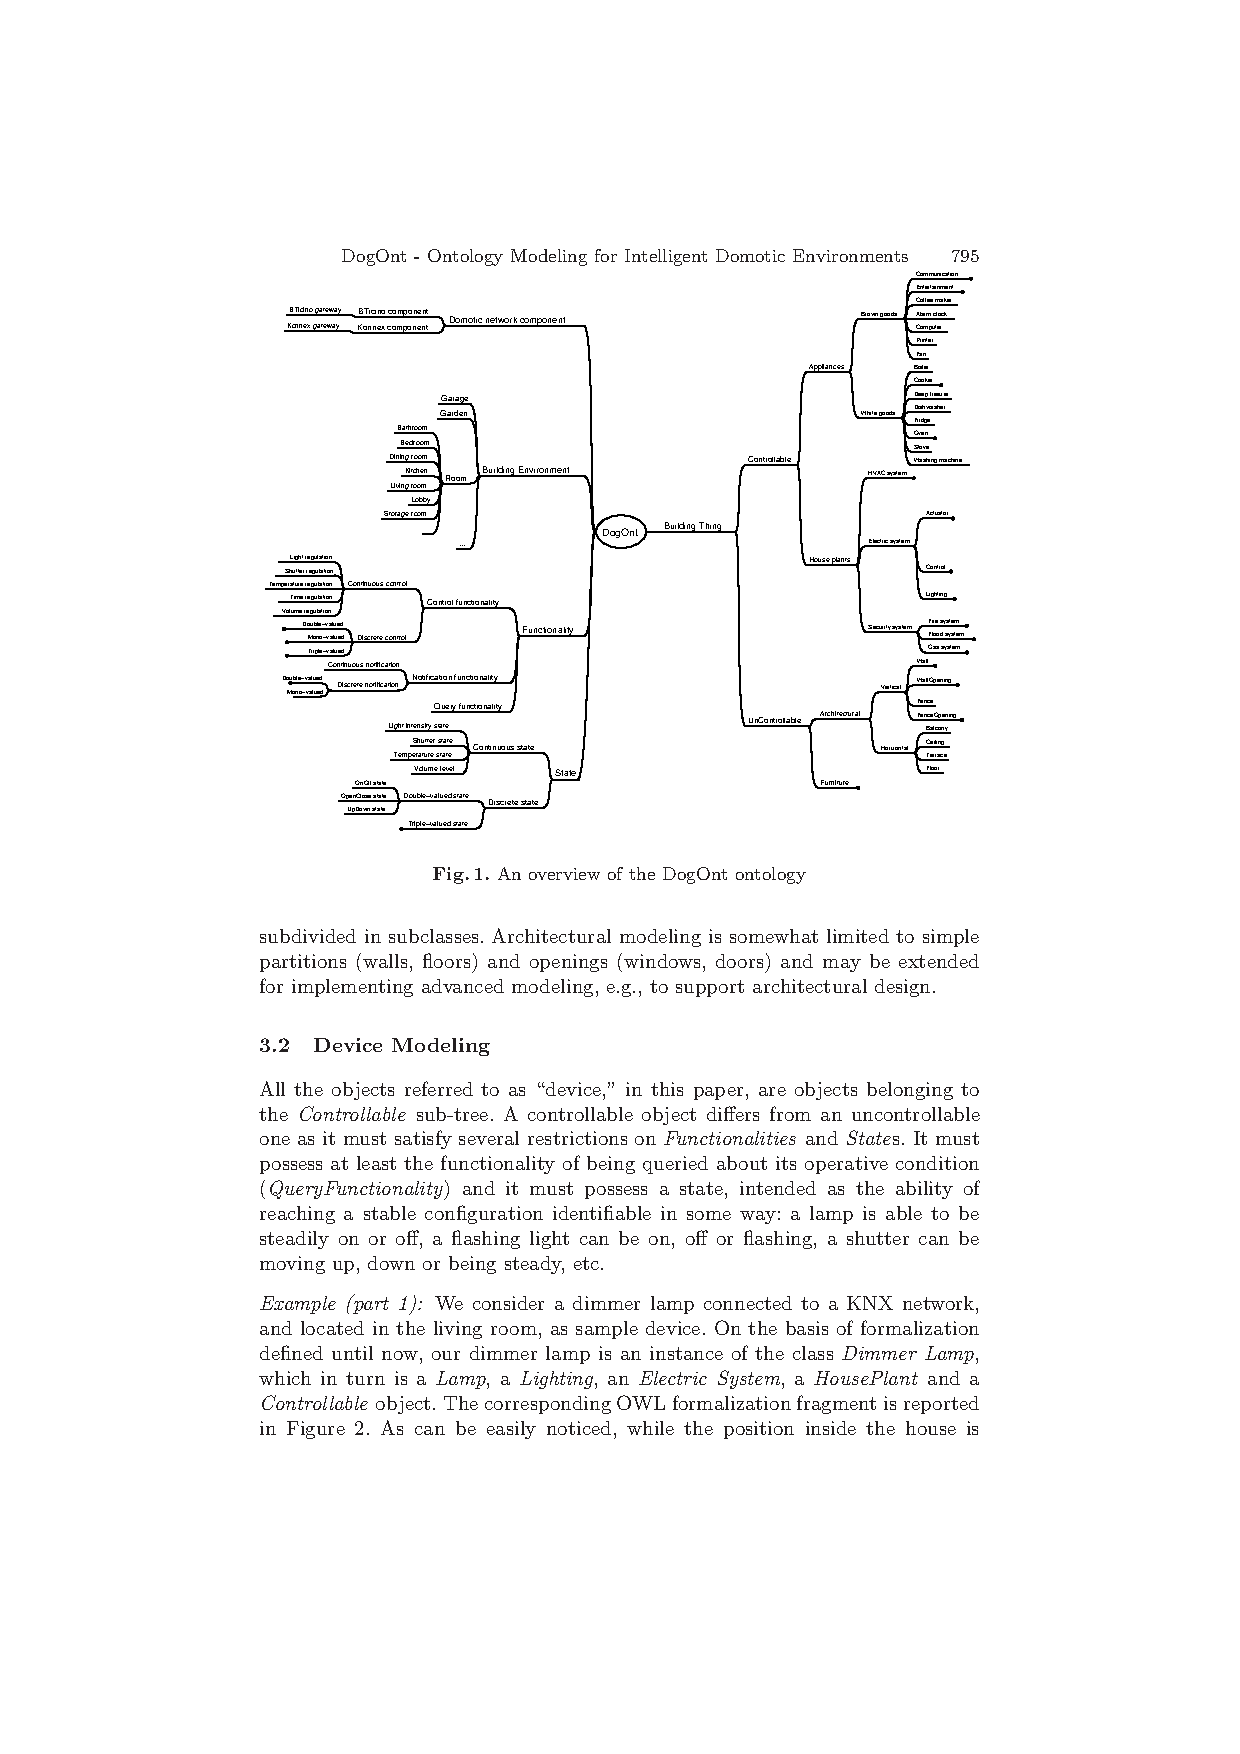
\includegraphics[width=0.8\textwidth, trim=4cm 15.5cm 4cm 4.6cm, clip]{rw-supervision-dogont}
    \caption{L'ontologie de DogOnt}\label{fig:rw:supervision:dogont}
\end{figure}
Pour pouvoir observer, et contrôler, les instances de ces concepts, il est nécessaire de rajouter des fonctionnalités et des variables d'états. Ceci se fait par l'introduction de relations sémantiques telles que \textit{hasControl}, \textit{hasFunctionality}, et \textit{hasState}. En combinant ces associations ainsi que l'ensemble complet des instances, il est possible de représenter l'ensemble des périphériques et leurs capacités.

Plusieurs autres projets ont utilisé ce type de modélisation pour des applications pervasives. Par exemple, Amigo~\cite{BenMokhtar:easy} se focalise plus sur la modélisation des services et des capacités. A contrario, \textit{MATCH}~\cite{Docherty:match} met l'accent sur la hiérarchie des ontologies pour que chaque domaine puisse apporter ses connaissances en utilisant des concepts communs (\textit{dispositifs}, \textit{réseau},\dots).

Nous remarquons que la séparation des domaines permet de gérer les perspectives utilisateurs en fonction de leurs intérêts. De plus, nous notons que l'hétérogénéité des schémas conceptuels est gérée par l'utilisation d'une ontologie commune. La nécessité d'une ontologie commune est récurrente dans ces travaux. Toutefois, dans des travaux récents~\cite{Niang:global,Niang:integration}, il existe des approches semi-automatiques pour intégrer des données de sources hétérogènes via la génération d'une ontologie commune et d'alignements.

\subsubsection{SOCAM : De l'utilité du raisonnement logique}
SOCAM (Service-Oriented Context-Aware Middleware)~\cite{Gu:socam} propose un intergiciel générique pour permettre aux développeurs de créer des applications pervasives par contexte. Cet intergiciel supporte l'acquisition, la découverte, l'interprétation et l'accès aux contextes. Comme les autres solutions présentées jusqu'ici, il s'appuie sur une ontologie conceptualisée comme celle de \textit{MATCH} afin de pouvoir être générique et y apporter les connaissances de chacun des domaines.

L'architecture de SOCAM, représentée en figure~\ref{fig:rw:supervision:socam} qui se décrit en trois 4 composants principaux.
\begin{figure}[ht]
    \centering
    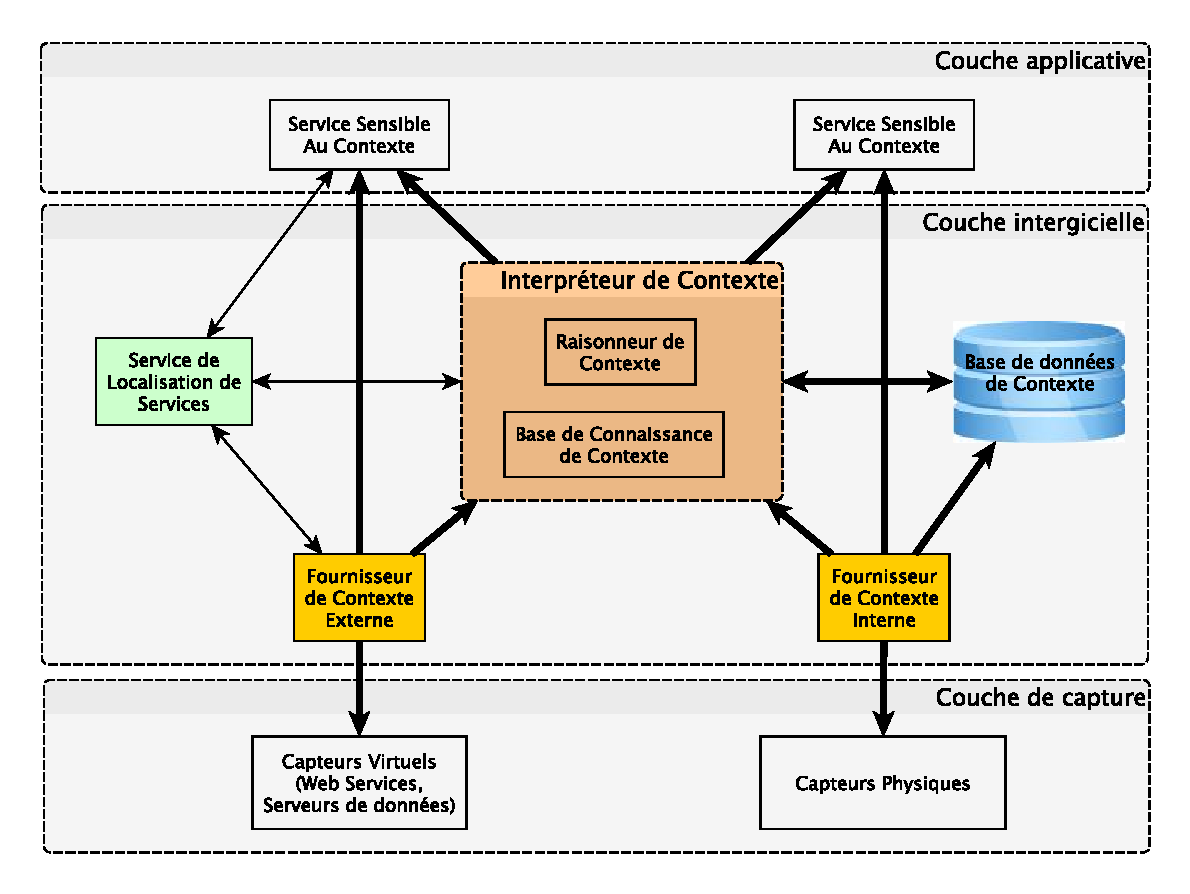
\includegraphics[width=0.66\textwidth]{rw-supervision-socam}
    \caption{Architecture de SOCAM}\label{fig:rw:supervision:socam}
\end{figure}
\begin{itemize}
	\item[\textbf{Fournisseurs de contexte}] Qui permet d'abstraire l'hétérogénéité des données issues des différentes sources (internes, tels que les capteurs ou autres dispositifs), ou externe (services météo ou autres) pour les convertir en \textit{OWL}.
    \item[\textbf{Interpréteur de contexte}] Fournit la logique de raisonnement sur le contexte.
    \item[\textbf{Base de données de contexte}] Stocke les ontologies de contexte et l'historique des contextes pour chaque sous-domaine.
    \item[\textbf{Service de localisation de services}] Sert de catalogue des services externes disponibles. Sa sélection peut se faire sur un type de service, mais il peut aussi faire une comparaison sur le contexte que le service fournit.
\end{itemize}
Les services applicatifs utilisant la notion de contexte vont ainsi utiliser les fonctionnalités que fournit SOCAM pour gérer cet ensemble de données. Une manière classique de construire ces services est de spécifier des actions déclenchées par un ensemble de règles au moment où le contexte change.

SOCAM implémente deux manières de faire de l'inférence logique de prédicats. La première est l'inférence structurelle. En effet, l'application d'une propriété transitive à un concept nous donne plusieurs informations. Par exemple, nous pouvons inférer que l'appareil \textit{Livebox} est une passerelle internet. Or, tous les équipements de cette catégorie ont des propriétés telles que la capabilité à gérer les règles de routage. La deuxième manière d'inférer des informations est un ensemble de règles utilisateurs. En utilisant un moteur similaire aux moteurs \textit{Prolog}, il est possible d'induire des informations qui constituent l'ensemble des situations. Par exemple, les auteurs présentent l'inférence du triplet \textit{(user socam:status 'SLEEPING')} par la détection de la position allongée dans la chambre avec la lumière éteinte.

Nous remarquons ici la présence d'une couche de traitement de données entre les sources et les services qui les utilisent. Cette couche se base sur des inférences logiques qui utilisent un support persistant pour constituer son contexte.

\subsection{Synthèse}
En conclusion, le traitement contextuel des données permet de gérer l'hétérogénéité sémantique des données. Les capacités de traitements sont liées à l'inférence logique pour enrichir la base des connaissances accumulées. Ainsi, il est possible de construire un espace de contexte et d'en inférer des situations de haut niveau. Cette capacité d'abstraction est nécessaire pour l'informatique ubiquitaire qui a besoin de manipuler des concepts humains.

Pour notre problématique d'observation, il reste difficile de gérer l'évolution des données au cours du temps. La liberté d'expression des bases de connaissances fait que l'inférence est complexe à manipuler. Plusieurs travaux s'attellent à permettre aux connaissances et aux règles d'introduire la dimension dynamique~\cite{Weikum:webknowledge, Hellerstein:declarative}. L'apport de cette dimension est toutefois difficile d'un point de vue théorique.

\begin{table}[!ht]
\criteretabDonnee
    {Structure sémantique à base de triplet.}
    {Utilisation d'ontologies. Gestion des contraintes et de l'inférence structurelles variable suivant l'expressivité du langage. En général, \textit{OWL Lite} est utilisé.}
    {Pas de gestion explicite du dynamisme en dehors d'annotations.}
\criteretabTraitement
    {Instantané uniquement.}
    {Les sources s'intègrent en se conformant à un modèle commun. Si tel n'est pas le cas de façon native, des règles d'alignements d'ontologies sont à fournir.}
    {Paradigme déclaratif en général dérivé de programmation logique allant de \textit{Prolog} à \textit{SPARQL}.}
    {Cela part de la logique du premier ordre complète à la capacité de l'algèbre relationnelle (\textit{datalog} non récursif avec négation)}
\criteretabAdaptabilite
    {Nécessité de spécifier des ontologies de domaines pour donner la structure des concepts du système.}
    {La séparation des domaines et le rattachement des données aux domaines permettent de clairement spécifier les différentes perspectives.}
    {Pas d'extensibilité possible sur le traitement d'inférence. Par contre, il est possible suivant l'architecture du système final de créer des capteurs de contextes pour fournir des données logiques de haut niveau.}
    {La complexité de l'inférence peut aller jusqu'en \textit{EXPTIME}. Toutefois, plusieurs implémentations optimisées permettent de traiter des millions de triplets en quelques secondes.}
\caption{Synthèse de l'informatique contextuelle}\label{tab:rw:supervision:contexte:synthese}
\end{table}

\section{Présentation des problématiques}\label{sec:intro:problematique}
Contrairement aux approches actuelles, nous considérons comme acquis le fait de pouvoir dialoguer d'une manière ou d'une autre avec le système pour récolter les données. La figure~\ref{fig:intro:objectif:abstraction} représente la couche d'abstraction du système, permettant un accès unifié aux données. Le système est donc considéré comme un ensemble de sources de données qu'il est nécessaire de maîtriser. Dans cette section nous présentons les problématiques soulevés par l'observation de systèmes génériques.

\begin{figure}[ht]
\centering
\includegraphics[width=0.7\textwidth]{intro-objectif}
\caption{Couche d'abstraction du système pour donner accès aux données}\label{fig:intro:objectif:abstraction}
\end{figure}

\subsection{Hétérogénéité des systèmes}
Plus l'informatique évolue, plus le nombre de dispositifs créés varie. Grâce à l'émergence de l'informatique ubiquitaire, les dispositifs se font de plus en plus nombreux et de natures complètement différentes. Ces caractéristiques rendent leur observation plus délicate car la surveillance des données d'un capteur est sensiblement différente à celle de l'utilisation d'un service d'hébergement web sur un serveur grande capacité.

Ainsi, il est nécessaire d'être capable de représenter toute sorte de système. Pour cela, il est nécessaire de définir un \textbf{schéma de données} reposant sur un \textbf{modèle de données}. Ce schéma détermine la sémantique accordé au système. Par exemple, en gestion de base de données, un modèle entité-relation détermine la représentation logique du système. Elle est par la suite traduite de façon physique en tables. En système d'information, la représentation d'un système passe souvent par un modèle objet. Cette capacité à représenter le système est critique pour manipuler clairement les concepts et leurs liens.

\subsection{Évolution des données du système}
Le système n'est pas statique dans le temps, c'est même souvent sa dynamique qui en fait sa richesse. Toutefois, cela introduit des problèmes majeurs d'un point de vue gestion des données. En effet, dans un système il existe deux grandes \textbf{catégories de données} : les données archivées et les données temps-réel. Les données archivés sont à évolution lente mais permet l'accès à des analyses de haut-niveau. Les données temps-réel sont des relevés instantanées et très volatiles indiquant l'état des entités du système (sous forme de flux de données).

Néanmoins, en l'état, chacune de ces catégories possède des modèles de données et des traitements propres. Or, ces données font toutes parties du même système. Nous pouvons remarquer qu'il existe des ponts naturels entre ces types. En effet, les approches classiques de surveillance par l'archive et l'analyse a posteriori montre qu'un flux nécessite d'être considéré comme un tout. De la même manière, une donnée stockée pourra subir des modifications déclenchant la production d'événements, assimilables à des flux de données.

La création des processus de traitements de données est assimilable à une interrogation que pose l'utilisateur sur l'ensemble des données. Il existe différentes \textbf{modes d'interrogations} (ou requêtes). Celles-ci reflètent l'hétérogénéité de l'évolution des données.
\begin{itemize}
    \item \textbf{Interrogation instantanée} : C'est la manière usuelle d'interroger dans les applications de gestion de base de données. L'utilisateur pose une question sur un ensemble de données considérées figées, du moins le temps du calcul de la réponse. Le système fournit une réponse représentative d'un état à un instant donnée. Un exemple simple étant : \enquote{\it quel est l'ensemble actuel des équipements actifs de mon système}. La réponse à cette requête pourrait être \enquote{\it à cet instant, les équipements Box, PC1 et STB sont connectés et actifs}. La mention \enquote{\it à cet instant} est très importante, car si un nouvel équipement arrive dans le système, une nouvelle évaluation donnerait une réponse différente. Ainsi, cette interrogation correspond à la consultation ponctuelle de l'ensemble des données disponibles.
    \item \textbf{Interrogation continue} : C'est l'élément principal des systèmes événementiels, où les données sont considérés en constante évolution. L'utilisateur obtient ainsi une réponse qui évoluera au cours du temps, sous forme de flux ou de mise à jour d'état. Un exemple pouvant être : \enquote{\it le flux de la charge processeur moyenne sur une minute du PC1}. La réponse forme un flux continu d'information qui, toutes les minutes, reporte une nouvelle valeur moyenne pour ce capteur. Ainsi, la formation de processus de collecte ou de formation d'alerte suivent ce type d'interrogation.
\end{itemize}

Il est important de noter que ces deux grands paradigmes d'interrogation peuvent se combiner. Par exemple, il est possible d'effectuer un appel à une interrogation instantanée à l'intérieur d'un processus continu. De façon similaire, l'appel régulier d'une interrogation instantanée forme une réponse continue. Il est donc nécessaire que le système d'observation soit capable de manipuler naturellement ces deux types d'interrogations pour manipuler correctement le dynamisme des données.

\subsection{Hétérogénéité des données et traitement}
La couche d'accès aux données permet d'exposer un ensemble de sources. Ces sources sont hétérogènes en terme de schéma et de nature (flux, archive).

Pour permettre une bonne compréhension du système et de ses interactions, il est nécessaire d'\textbf{intégrer} les différentes sources d'informations en une seule base d'information. En effet, chaque source de donnée peut-être considérée comme un fragment de cet ensemble. Ainsi, le système doit se doter de fonctionnalités d'agrégations de plusieurs sources.

L'\textbf{expression} des traitements possibles se fait à travers d'un \textbf{langage}. Son paradigme sous-jacent définit la manière et la facilité d'adaptation à un système en particulier. Ce langage peut être dans le cas le plus extrême : un langage de programmation impératif bas niveau (comme le C par exemple). Dans ce cas, l'approche est très algorithmique, permettant une meilleure gestion des performances, mais une utilisation plus difficile et technique par la suite. À l'autre extrême, le langage peut être issu de la programmation logique permettant des performances moins contrôlées, mais une gestion globale déclarative, permettant une grande flexibilité.

Le langage utilisé dans le système d'observation peut avoir un \textbf{pouvoir d'expression} limité. Il est important d'être capable d'énumérer ce qui est possible, ou non, d'exprimer en terme de processus. Les classes de logiques ou les équivalences à d'autres langages permettent de caractériser ces limitations. Par exemple, les opérations de manipulation de données pourrait être limitées par la logique du premier ordre, ou par le calcul relationnel.

\subsection{Adaptabilité à l'application}
Le point critique de mise en œuvre d'un système d'observation est sa capacité à s'adapter à l'application finale. Plus la portée de l'observation est générique plus ce critère est important. Ainsi, il est nécessaire que le nombre et la complexité des procédures nécessaires à l'adaptation au système visé soit faible. Car si un système est complet mais nécessite une adaptation longue et complexe, il devient difficile à mettre en pratique.

L'observation ne se justifie que par l'utilisation qui en est faite et par son application. En effet, pour tout système, il existe plusieurs \textbf{perspectives} possibles. Cet angle définira par la suite les données surveillées mais aussi la représentation du système. Il est nécessaire que le système d'observation s'adapte aux perspectives dans lesquelles se placent les experts.

Afin de pouvoir s'adapter aux besoins des experts. Il est ainsi nécessaire que le système d'observation soit capable d'\textbf{intégrer des routines spécifiques} de traitement de données. Cette extensibilité permet aussi bien l'intégration de tous types de besoins que l'amélioration des performances de traitements récurrents.

Enfin, pour que l'observation puisse être déployable dans le plus grand nombre de contextes différents, il est nécessaire que le système d'observation soit efficace. De plus, ce critère améliore la qualité des réponses aux différentes requêtes de l'utilisateur. En effet, l'amélioration des performances permet la réduction des coûts de temps de traitement. La réponse devient ainsi disponible plus rapidement et reflète une vision plus à jour des données. Le critère se mesure sur la capacité à traiter la charge d'un système en terme de nombre de sources ou en terme de débit supportés.


\section{Une supervision générique orientée données}\label{sec:intro:objectif}
Il existe de nombreux produits commerciaux ou académiques de supervision pour effectuer des taches de surveillances notamment dans le cadre de la gestions de serveurs (d'un point de vue réseau~\cite{gestion équip réseau} ou applicatif~\cite{supervision apache}), la gestion de processus opérationnels d'entreprises~\cite{google:business process supervision} et l'administration d'un parc de dispositifs~\cite{snmp:voir thèse mehdi}. Cependant, les approches actuelles ont différents problèmes majeurs :
\begin{itemize}
    \item \textbf{Restriction à une perspective} : comme vu précédemment, la supervision doit s'adapter aux différents systèmes et aux différents angles de vues possibles. Plusieurs solutions ne se focalisent que sur un cœur de métier en particulier, rendant l'ensemble très ad-hoc et peu réutilisable.
    \item \textbf{Vision unilatérale} : l'observation ne se fait que sur une seule entité du système (un ensemble de données d'un équipement). Le système n'est pas considéré comme un tout rendant la compréhension des interactions entre les entités du système difficile.
    \item \textbf{Focalisation forte sur le processus de collecte} : en l'état, beaucoup de travaux ont été effectués pour permettre aux solutions d'administrations d'accéder aux équipements. Ceci certes permet l'accès aux données mais ouvre la porte à une gestion difficile de la grande quantité ainsi obtenue.
    \item \textbf{Gestion de l'évolution des données limitée} : deux approches principales sont utilisées en l'état. Soit le traitement des données se fait \textit{à chaud} par l'observation d'une fenêtre de temps limitée permettant ainsi de favoriser les solutions proactive pour notamment faire des systèmes d'alerte. Soit les données sont archivées pour en faire le traitement plus complexe par la suite en vu d'une analyse plus poussée. Il est très rare de voir un système d'observation capable de gérer ces deux approches de façon unifiée. 
\end{itemize}
\begin{figure}
\centering
\includegraphics[width=0.7\textwidth]{fig/intro-objectif.eps}
\caption{Couche d'abstraction du système pour donner accès aux données}\label{fig:intro:objectif:abstraction}
\end{figure}

L'objectif final de cette thèse est d'obtenir une supervision générique permettant de répondre à la grande hétérogénéité présentée en section~\ref{sec:intro:problematique}. Contrairement aux approches actuelles, il est ici considéré comme acquis le fait de pouvoir dialoguer d'une manière ou d'une autre avec les dispositifs de manière à récolter les données. La figure~\ref{fig:intro:objectif:abstraction} représente la couche d'abstraction du système, permettant un accès unifié aux données. Le système est donc considéré comme un ensemble de sources de données hétérogènes qu'il nous faut maîtriser. Chacune de ces sources exposant un fragment de l'ensemble des données du système. Ce positionnement est principalement motivé par la grande quantité de travaux effectués sur le sujet et du fait que les dispositifs, même grand publique, permettent de plus en plus des accès standards à leurs canaux de données. Ainsi, cette thèse n'aborde pas les problématiques (complexes) d'hétérogénéité de protocoles de communications pour permettre l'accès aux données.

Ainsi, cette gestion de données sera l'interface entre le système à observer et les différents utilisateurs (humains ou machines). Ce système permettra ainsi de créer des processus de collecte et d'analyse de manière le plus flexible possible. Voici les caractéristiques que la solution se doit de respecter :
\begin{itemize}
    \item \textbf{Applicable sur tout type de système} : l'approche ne doit pas considérer comme acquis un type de système ou un cœur de métier en particulier. En effet, comme présenté précédemment, un des problèmes majeurs rencontrés dans les solutions existantes est la restriction à une perspective.
    \item \textbf{Un langage unifié} : il est nécessaire que les processus de traitement des données doivent être écrits dans un seul et même langage. Ce langage doit être capable de traiter l'hétérogénéité sur les données, y compris au niveau temporelle. En effet, le système de supervision mêlera données statiques et dynamiques sur lesquelles serons exécutés des traitements continus ou instantanés, le langage doit être capable d'exprimer proprement ces processus.
    \item \textbf{Performant} : l'exécution des processus doit pouvoir se faire de manière suffisamment efficace. L'aspect performance est à considéré car que ce soit pour le passage à l'échelle ou à l'inverse le déploiement sur dispositifs embarqué, la quantité de ressources nécessaire pour exécuter un processus doit être contrôlé.
    \item \textbf{Extensible} : si l'utilisateur souhaite pouvoir implémenter une nouvelle fonctionnalité, il doit avoir la possibilité de le faire. Ceci peut avoir un impact pour pouvoir par exemple effectuer un traitement spécifique à un métier, ou encore pour améliorer les performances dans un cadre particulier. Ainsi, il sera plus facile d'intégrer le système de supervision avec son cadre d'utilisation.
\end{itemize}

\section{Démarche et contribution de cette thèse}\label{sec:intro:demarche}
Nous proposons une approche orientée données pour l'observation de système. En particulier, nous avons choisi l'approche de la gestion des flux de données afin de : créer un langage algébrique unique d'interrogation pour toutes les catégories de données ; concevoir un intergiciel capable de gérer les données issus de l'observation de façon uniforme. Cette section présente brièvement nos contributions.

\subsection{Un langage unique d'interrogation}
La gestion de flux de données est un domaine permettant de gérer de manière déclarative les données temps-réel. Cette approche permet une grande souplesse car il est possible de déployer des requêtes complexes via un langage déclaratif sur les données. Toutefois, les langages manquent encore de fondations théoriques pour correctement maîtriser ses données.

Nous avons spécifié une algèbre permettant d'interroger de manière unifiée les données sous forme de flux ou relations de bases de données. Elle a pour propriété d'être capable de manipuler les deux modes d'interrogations sur des données archivés ou temps-réel. De plus, ses définitions sont entièrement déterministe ne laissant pas de place à l'interprétation, ce qui permet une gestion plus claire de ses données.

\subsection{Un intergiciel extensible d'évaluation de requête}
Il existe plusieurs intergiciels capables d'évaluer des requêtes continues sur les SGFD. Toutefois, leur implémentation peut influencer les sémantiques d'évaluations de requête. Des approches existent pour intégrer des évaluateurs d'un point de vue architectural. Toutefois, il existe peu d'approche pour spécifier formellement le comportement d'un opérateur d'un évaluateur.

Nous proposons un intergiciel capable d'évaluer des requêtes exprimés dans le langage algébrique que nous avons développé. Cette algèbre nous sert aussi pour la spécification des composants de l'intergiciel. En effet, chaque module implémentant un opérateur doit spécifier sa sémantique selon une ou plusieurs règles se basant sur des opérateurs algébriques. Ce principe couplé avec les notions architecturales de composants orientés services nous permettent d'avoir une grande flexibilité pour permettre aux utilisateurs de personnaliser au mieux cette solution.

De plus, notre approche à base de règle nous permet de développer une approche générale d'optimisation des requêtes. Tout comme en SGBD, nous appliquons une optimisation logique, puis physique de notre requête. Ces optimisations sont possibles grâce aux résultats d'équivalence de requête démontrable avec l'algèbre.

\subsection{Une intégration des supports persistants}
Enfin, nous avons vu que notre langage est capable d'interroger de manière unifié les données temps-réel et archivés. Dans la littérature, plusieurs existent entre les deux mondes de manière ad-hoc ou implicite.

Grâce à notre langage, nous proposons une infrastructure capable d'intégrer un SGBD à notre intergiciel. Ainsi, l'utilisateur doit spécifier son schéma contextuel précisant sa représentation du système, ainsi que des requêtes permettant l'intégration des données flux dans la base. À l'issue de ce travail de spécifications, l'utilisateur devient capable d'interroger les données archivés et temps-réel via l'algèbre. Il est alors garanti de la mise en œuvre de sa requête de façon efficace. Cette infrastructure est proposé comme extension de notre intergiciel.

\section{Plan de thèse}\label{sec:intro:plan}
Ce manuscrit est découpé en trois parties majeures :
\begin{enumerate}
\item \textbf{L'état de l'art}. Nous analysons d'abord les solutions actuelles capables de faire de l'observation de systèmes génériques dans le chapitre~\ref{chap:rw:supervision}. Ensuite, nous détaillons les travaux existant dans le domaine plus spécifique de la gestion des flux de données dans le chapitre~\ref{chap:rw:sgfd}.
\item \textbf{Contribution}. Le chapitre~\ref{chap:contrib:astral} présente les définitions d'\textit{Astral}, notre algèbre de gestion de données. Le chapitre~\ref{chap:contrib:astronef} décrit \textit{Astronef}, un intergiciel capable d'interpréter et évaluer une requête \textit{Astral}. Enfin, nous détaillons dans le chapitre~\ref{chap:contrib:asteroid} l'extension capable de manipuler un support persistant relationnel, complétant ainsi notre gestion de données pour l'observation.
\item \textbf{Validation et mise en pratique}. Le chapitre~\ref{chap:validation:expressivite} analyse en détail l'expressivité offerte par \textit{Astral}, en la comparant à l'état de l'art, puis en démontrant des propriétés non-triviales d'équivalences de requêtes. La mise en œuvre de notre solution d'observation dans le cadre du réseau local domestique est décrite dans le chapitre~\ref{chap:valid:domvision}. Dans ce chapitre, nous introduisons aussi un nouvel opérateur permettant de gérer les préférences utilisateurs pour montrer la flexibilité de l'intergiciel. Puis, nous présentons dans le chapitre~\ref{chap:valid:perfs} des éléments d'évaluation de performances afin de démontrer que notre système de règle permet d'évaluer de manière efficace : des requêtes continues, des requêtes couplés avec un SGBD et des requêtes impliquant un opérateur introduit par l'utilisateur.
\end{enumerate}

Finalement, le chapitre~\ref{chap:conclusion} conclut ce travail et présente quelques perspectives de recherches.
